\documentclass[Modultest/Modultest_main.tex]{subfiles}
\begin{document}
\section{GameController}\label{sec:test_Game}
I dette afsnit beskrives modultesten af GameController. GameController er controller modulet for RPiApp. Generelt er det svært at modelteste GameController, da den ikke har en entydig opgave. Med det sagt er der nogle operationer som er kritisk for at klasserne kan kommunikere med hinanden: 
\begin{enumerate}
    \item Test af MsgQueue kommunikation (Producer / Consumer)
    \item UserInfo instanser og logiske operationer 
\end{enumerate}
\subsection{Test af MsgQueue kommunkation}
Det essentielle for programmet er den trådsikre kommunikation. For at teste systemet, skal der sendes beskeder til GameController. Dette gøres ved at dynamisk allokere bruger definerede beskeder, som sendes til GameControllers MsgQueue instans. Dispatcheren afvilker det som sendes til MsgQueuen sekventielt. Den modtager et MsgId, som identificerer den service som 'requestes', kalder tilhørende handler og static\_cast'er beskeden til den korrekt type nedarvning. \\\\
Denne metode benævnes som "White-box testing", som tester de interne strukturer og funktionsmåder i applikationen, i modsætning til dets funktionalitet ("Black-box").\autocite{Whitebox}\\\\
Der bruges White-box testing, da det er essentielt for programmet at den interne kommunikation mellem tråden er operationel og virker optimalt. 
Først simuleres indsættelse af en mønt. Her gøres brug af en brugerdefineret besked, som indeholder en const char pointer til det som reelt er sendt til GameControllers MsgQueue fra BallDispenserRead. \\
Brugerdefineret besked: 
\begin{lstlisting}
class BallDispenserResponse : public Message
{
public:
	BallDispenserResponse(const char * readPtr)
	    : readPtr_(readPtr)
	{}
	const char * readPtr_;
};
\end{lstlisting}
Simulering af møntindsættelse (Her gøres brug af prædefineret protokol kommandoer defineret i MsgProtokol).: 
\begin{lstlisting}
GameController::handleIdleRequest()
{
...

GameControllerMsgQueue_->send(BallDispenser::NEW_INFO, new
BallDispenserResponse(&BallDispenserMessage.COIN_INSERTED));
}
\end{lstlisting}
GameeController initiere stadiet "IDLE" ved at sende en besked til sin egen MsgQueue. Her kaldes handleIdleRequest, hvor en mønt simuleres som vist ovenfor. \\\\
Der indsættes kommentar i den store switch case for GameController, således det kan kontrolleres at de korrekte cases bliver kaldt: 
\begin{lstlisting}
void GameController::dispatcherGameMessage(unsigned long msgID, Message * msg)
{
	switch (state)
	{
	case GAME_STATE_IDLE:
	{
		switch (msgID)
		{
		case SYSTEM_STATE::IDLE:
		{
			cout << "SYSTEM_STATE::IDLE" << endl;
			handleIdleRequest();
		}
		break;

		case BallDispenser::NEW_INFO:
			cout << "NEW_INFO : ";
			handleBallDispenserResponse
			(static_cast<BallDispenserResponse *>(msg));
		break;
    ...
\end{lstlisting}

\subsubsection{Resultater}
\begin{figure}[H]
    \centering
    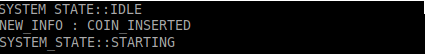
\includegraphics[width=\textwidth]{Modultest/GameController/graphic/Modeltest.png}
    \caption{Terminal output - Modultest for GameController}
    \label{fig:test_game}
\end{figure}

\subsubsection{Refleksion}
Trådkommunikationen med MsgQueue er nu testet og operationelt. Så længe alle klasser sender dynamiske beskeder og allokerer beskederne statisk efter korrekt type nedarvning, bør der ikke opstå fejl allokering af resourcer eller segmentation faults.

\subsection{PlayersideWrite og PlayersideRead Modultest}
Dette afsnit testes PlayersideWrite og PlayersideRead filoperationerne og den prædefineret protokol angivet i klassen MsgProtocol. Trådkommunikationen er 'bekræftet' i modultesten for GameController, så den bruges til at sende beskeder til PlayersideWrite og -Read for at teste at det korrekte kan sendes til PSoC enhederne. \\\\
\textbf{White-Box test fremgangsmåde - 'Flow'}
\begin{enumerate}
    \item GameController kalder funktion handleIdleRequest(), som sender en stadiekommando til PlayersideWrite: 
    \begin{lstlisting}
    PlayersideWriteObj1_->
    PlayersideMsgQueue_.send(SYSTEM_STATE::IDLE);
    \end{lstlisting}
    \item PlayersideWrite modtager beskeden og afvikler den: 
    \begin{lstlisting}
    ... //Inside Switch case // ... 
    case SYSTEM_STATE::IDLE :{
	cout << "PS_WRITE" << playerside_ 
	<< ": STATE IDLE" << endl;
	char sendBuffer[2] = {PlayersideMessage.IDLE};
	writePlayerside(sendBuffer, 1); 
    \end{lstlisting}
\end{enumerate}
\begin{figure}[H]
    \centering
    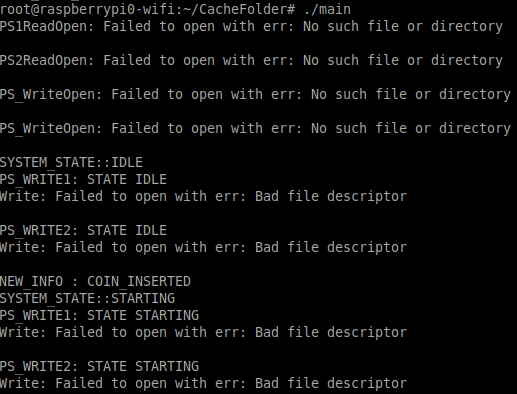
\includegraphics[width=\textwidth]{Modultest/GameController/graphic/Modultest_ps.png}
    \caption{Terminal output - Modultest for playerside read og write}
    \label{fig:test_playerside}
\end{figure}
\subsubsection{Refleksion}
Det kan ses at trådkommunikation virker som forventet og de korrekte funktioner bliver kaldt. Da der bruges fil-operationer for både read- og writemetoderne, vil vi modtage fejlbeskeder, da filerne ikke er oprettet og driveren er ikke integreret med programmet endnu - dette skal først undersøges ved integrationstesten med driveren og Playerside-enheden. 
Der laves ikke en modultest for BallDispenserRead og -Write, da der bruges samme operationer som PlayersideRead og -Write. 
\subsection{UserInfo modultest}
I dette afsnit beskrives modultesten for nogen af UserInfo operationerne, specifikt anvendelse af datamemberen \textbf{Cups\_}. \textbf{Cups\_} symboliserer antal kopper for hvert hold. Det er valgt at bruge biblioteket <bitset> for omdanne den char som modtages fra PlayersideRead til et array bools, såledet Display klassen let kan se hvilke kop som er blevet ramt, fx ved at bruge en index operator. \\\\
Der laves et lille testprogram for at teste funktionaliteten: 
\begin{lstlisting}
#include <bitset>
#include <iostream>
using namespace std;
//Prototype
bitset<6> setCups(const char * cupsArray)
{
	bitset<6> cups_; 
	cups_ = (bitset<6>)*cupsArray; 
	return cups_; 
}

enum {
	IDLE = 48, 
};

int main()
{
	bitset<6> cups_;
	//? = All cups placed = 0b00111111
	const char Array = '?'; 
	cups_ = setCups(&Array); 
	cout << "Cups: " << cups_ << endl; 

	cout << "sendbuffer: " << (unsigned char) IDLE << endl; 
	
	while(true) {}

	return 0; 
}
\end{lstlisting}
\subsubsection{Resultater}
\begin{figure}[H]
    \centering
    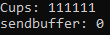
\includegraphics[width=0.6\textwidth]{Modultest/GameController/graphic/Modultest_userInfo.png}
    \caption{Terminal output - Modultest af bitset Cups\_ datamember}
    \label{fig:test_cups}
\end{figure}
\subsubsection{Refleksion}
Testning af denne funktion er måske lidt triviel, men det gør behandlingen af \textbf{Cups\_} lettere for Display klassen, og det bekræfter at man kan omdanne en char til et bitset array - bitset objekter har bl.a. også en del overloaded operationer og metoder, som bruges i GameController. 
\end{document}